\newpage
\appendix
\section*{Appendices}
\section{Original data and results PGExplainer}\label{appendix:A}

% \begin{table}[h]
%     \centering
%     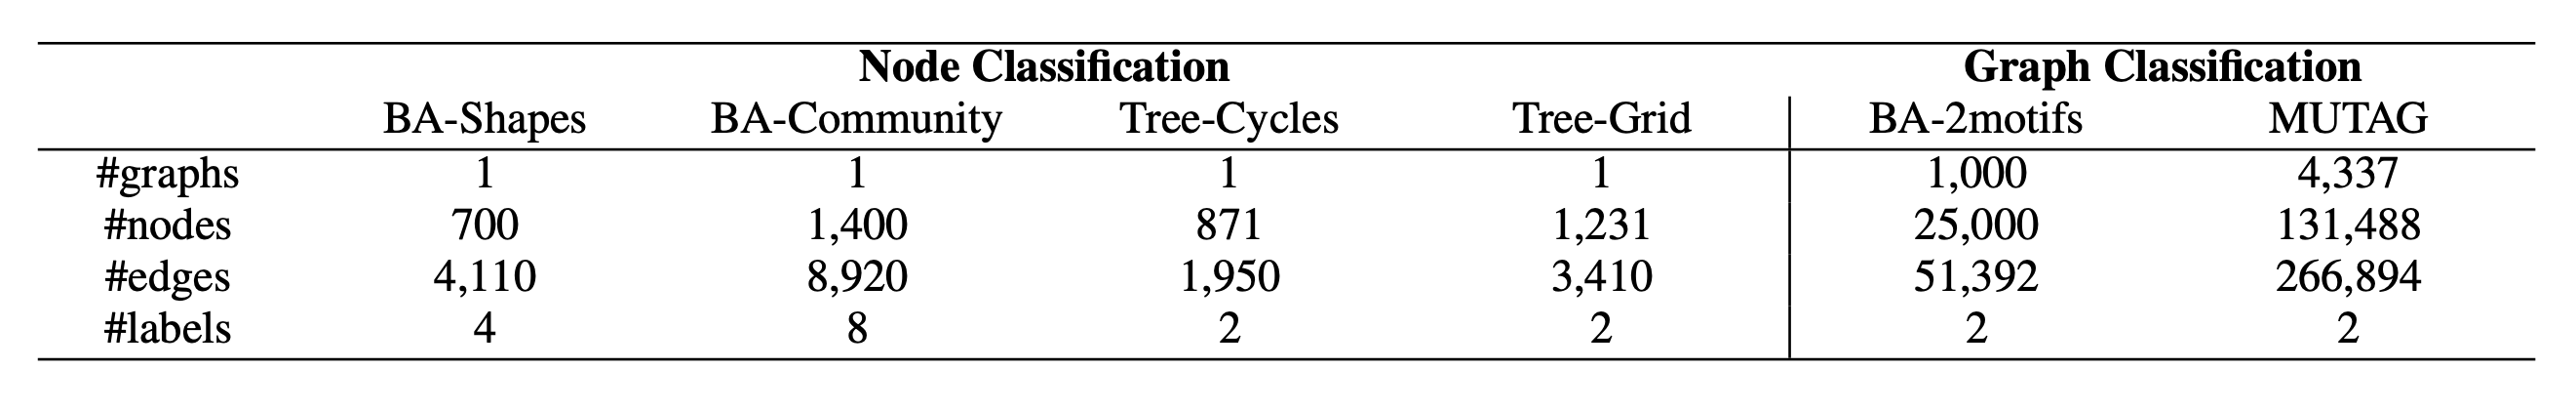
\includegraphics[width=1\linewidth]{imgs/dataset_info.png}
%     \caption{Original paper's dataset statistics \cite{luo2020parameterized}}
%     \label{tab:dataset_info}
% \end{table}

\begin{table}[h]
    \centering
    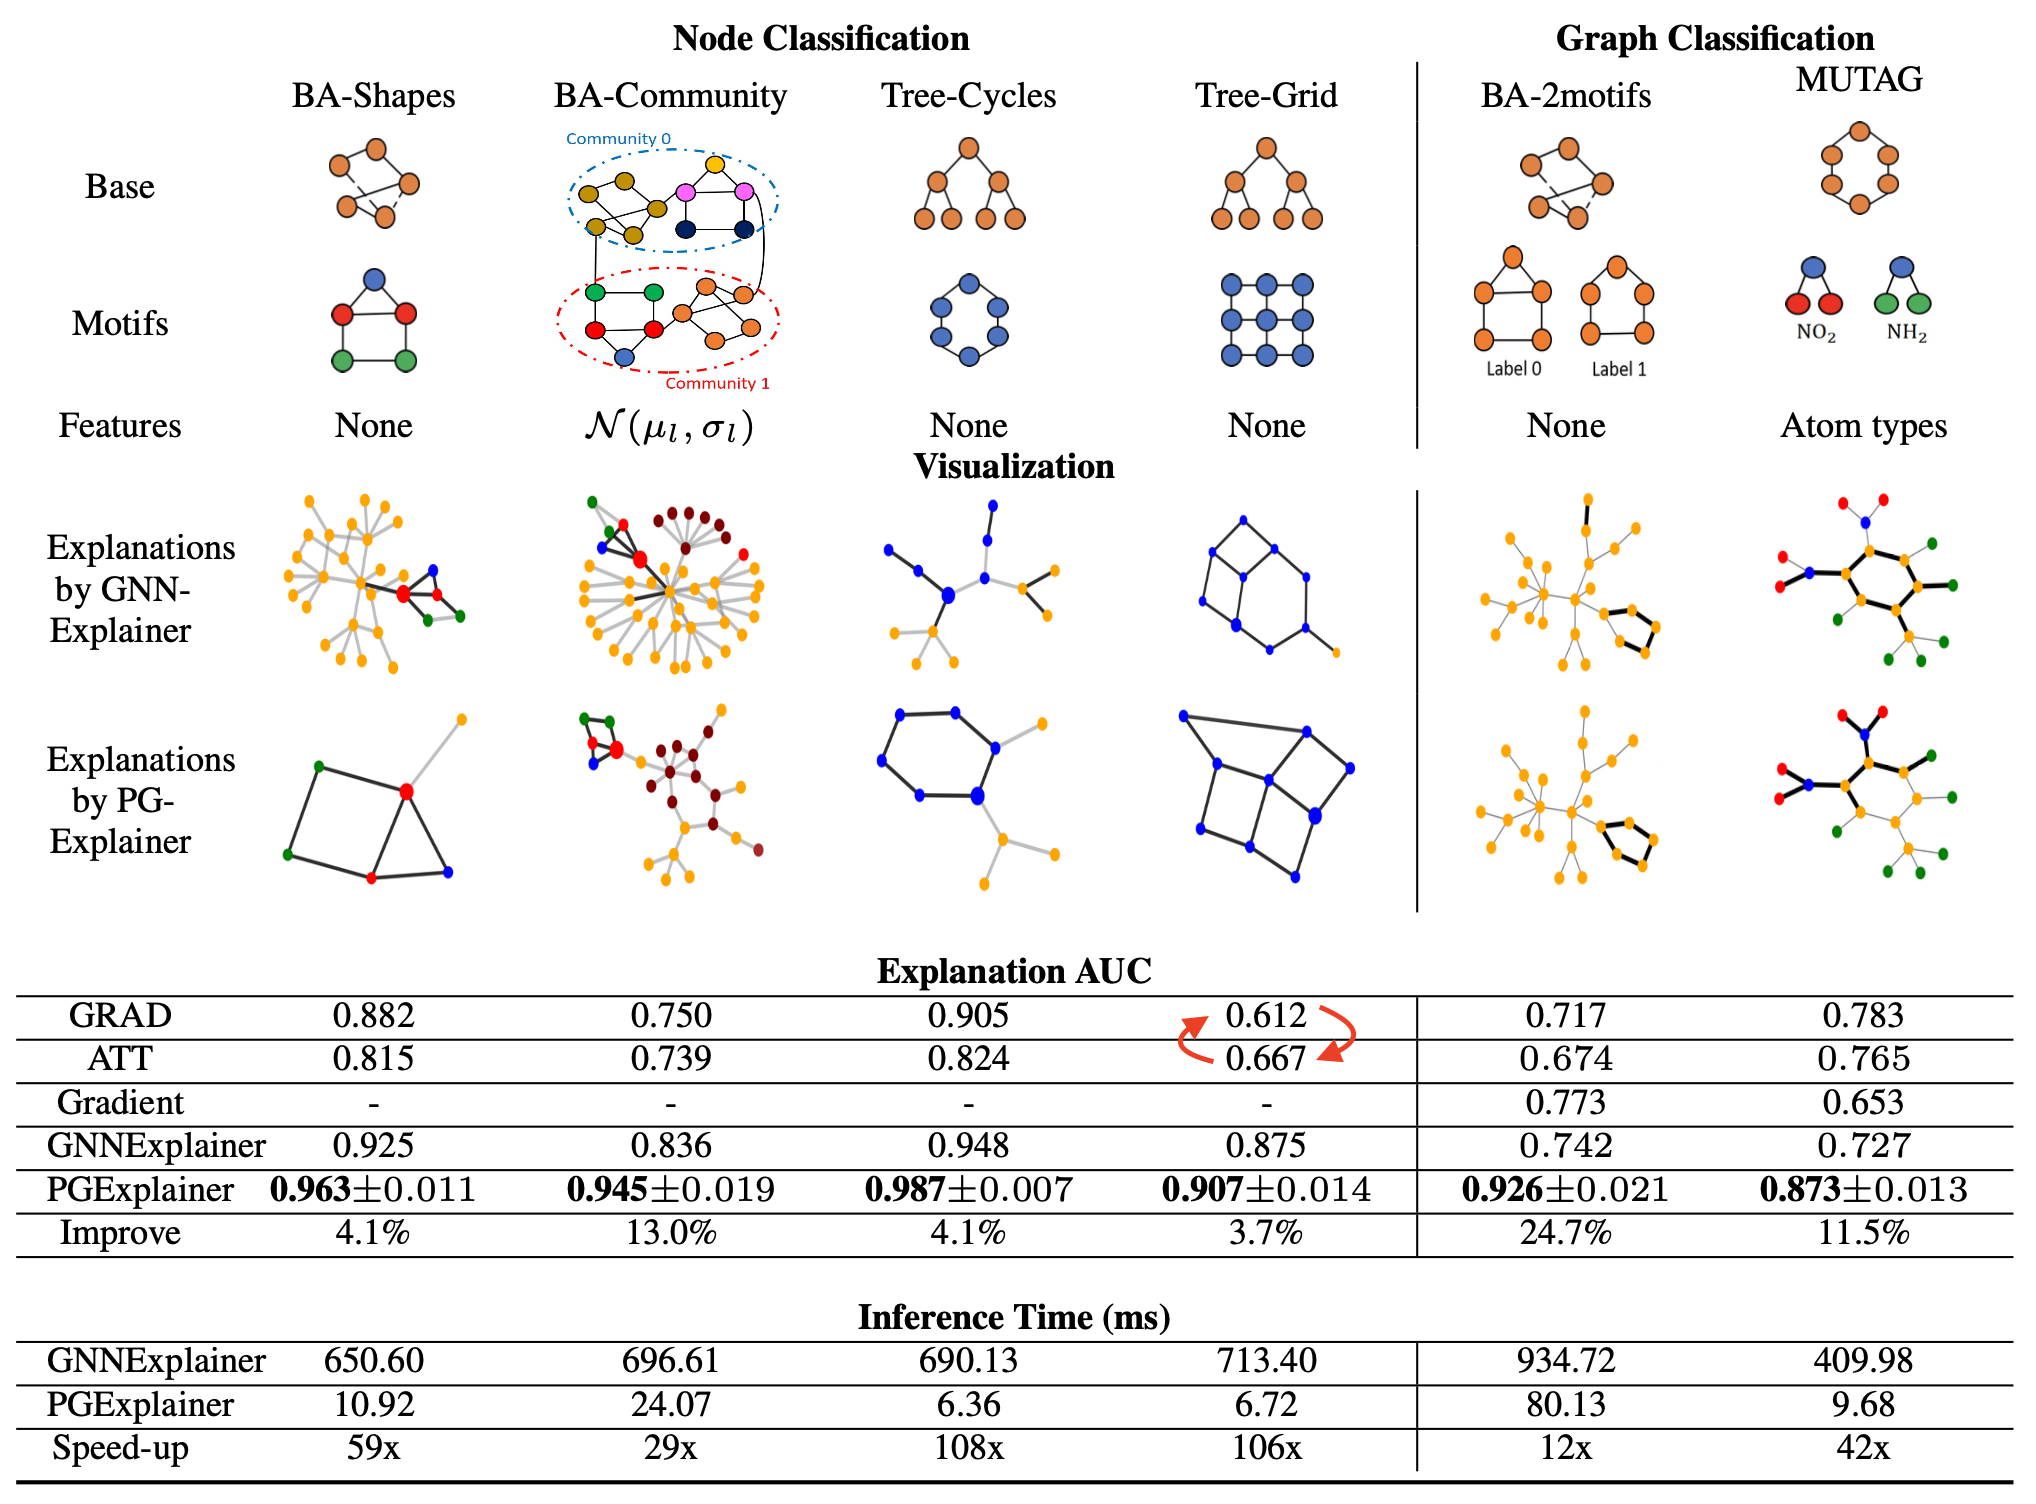
\includegraphics[width=1\linewidth]{../openreview/imgs/results2.png}
    \caption{Visual representations of the datasets, results and the performance evaluations \cite{luo2020parameterized}. \textbf{Note: The AUC scores for \textit{GRAD} and \textit{ATT} inside Tree-Grid are incorrectly copied by the authors and should be swapped (as indicated by the red arrows).}}
    \label{tab:results}
\end{table}

\section{Direct replication of PGExplainer with BatchNorm activated model} \label{appendix:batch_norm}
Here we present a replication experiment similar to the one presented in our replication work. However, as discussed in in the main work, the models used in the original paper contained two batch-normalization layers. These layers were incorrectly kept in training mode during evaluation. In the replication results presented here, the same batch-normalization setup was used for the node-classification models. 

\subsection{Results}
\paragraph{Model training}
Tab.\,\ref{tab:accuracies} shows that the accuracies of the models trained using the batch normalization are very similar to those used in the main paper. The BA-Community dataset still shows the same issues with overfitting as are discussed in the main paper. 

\begin{table}[]
\centering
\begin{tabular}{cccccc}
\toprule
&\multicolumn{4}{c}{\textbf{Node Classification}} \\
Accuracy & \multicolumn{1}{c}{BA-Shapes} & \multicolumn{1}{c}{BA-Community} & \multicolumn{1}{c}{Tree-Cycles} & \multicolumn{1}{c}{Tree-Grid}  \\ 
\midrule
Training & 0.98 & 0.94 & 0.96 & \multicolumn{1}{c}{0.96}  \\
Validation & 0.99 & 0.74 & 0.99 & \multicolumn{1}{c}{0.98}  \\
Testing & 1.00 & 0.71 & 0.97 & \multicolumn{1}{c}{0.99} &  \\
\bottomrule
\end{tabular}
\caption{Accuracies for models trained with batch-normalization. For evaluation of the validation and test dataset batch-normalization is kept in training mode. This is similar to the original paper. }
\label{tab:accuracies}
\end{table}

%                 Node classification                         Graph classification
%               Syn1, syn2m= .....                      Ba2, mutag
% -----
%visualization
%------
% PG them auc
% PG us auc
% ----
% inference time
\begin{table}[]
\centering
\begin{tabular}{lllll}
\toprule
\multicolumn{5}{c}{\textbf{Node Classification}} \\
\multicolumn{1}{c}{} & \multicolumn{1}{c}{BA-Shapes} & \multicolumn{1}{c}{BA-Community} & \multicolumn{1}{c}{Tree-Cycles} & \multicolumn{1}{c}{Tree-Grid} \\ \hline
\multicolumn{5}{l}{\textbf{Visualization}} \\ \hline
Original &  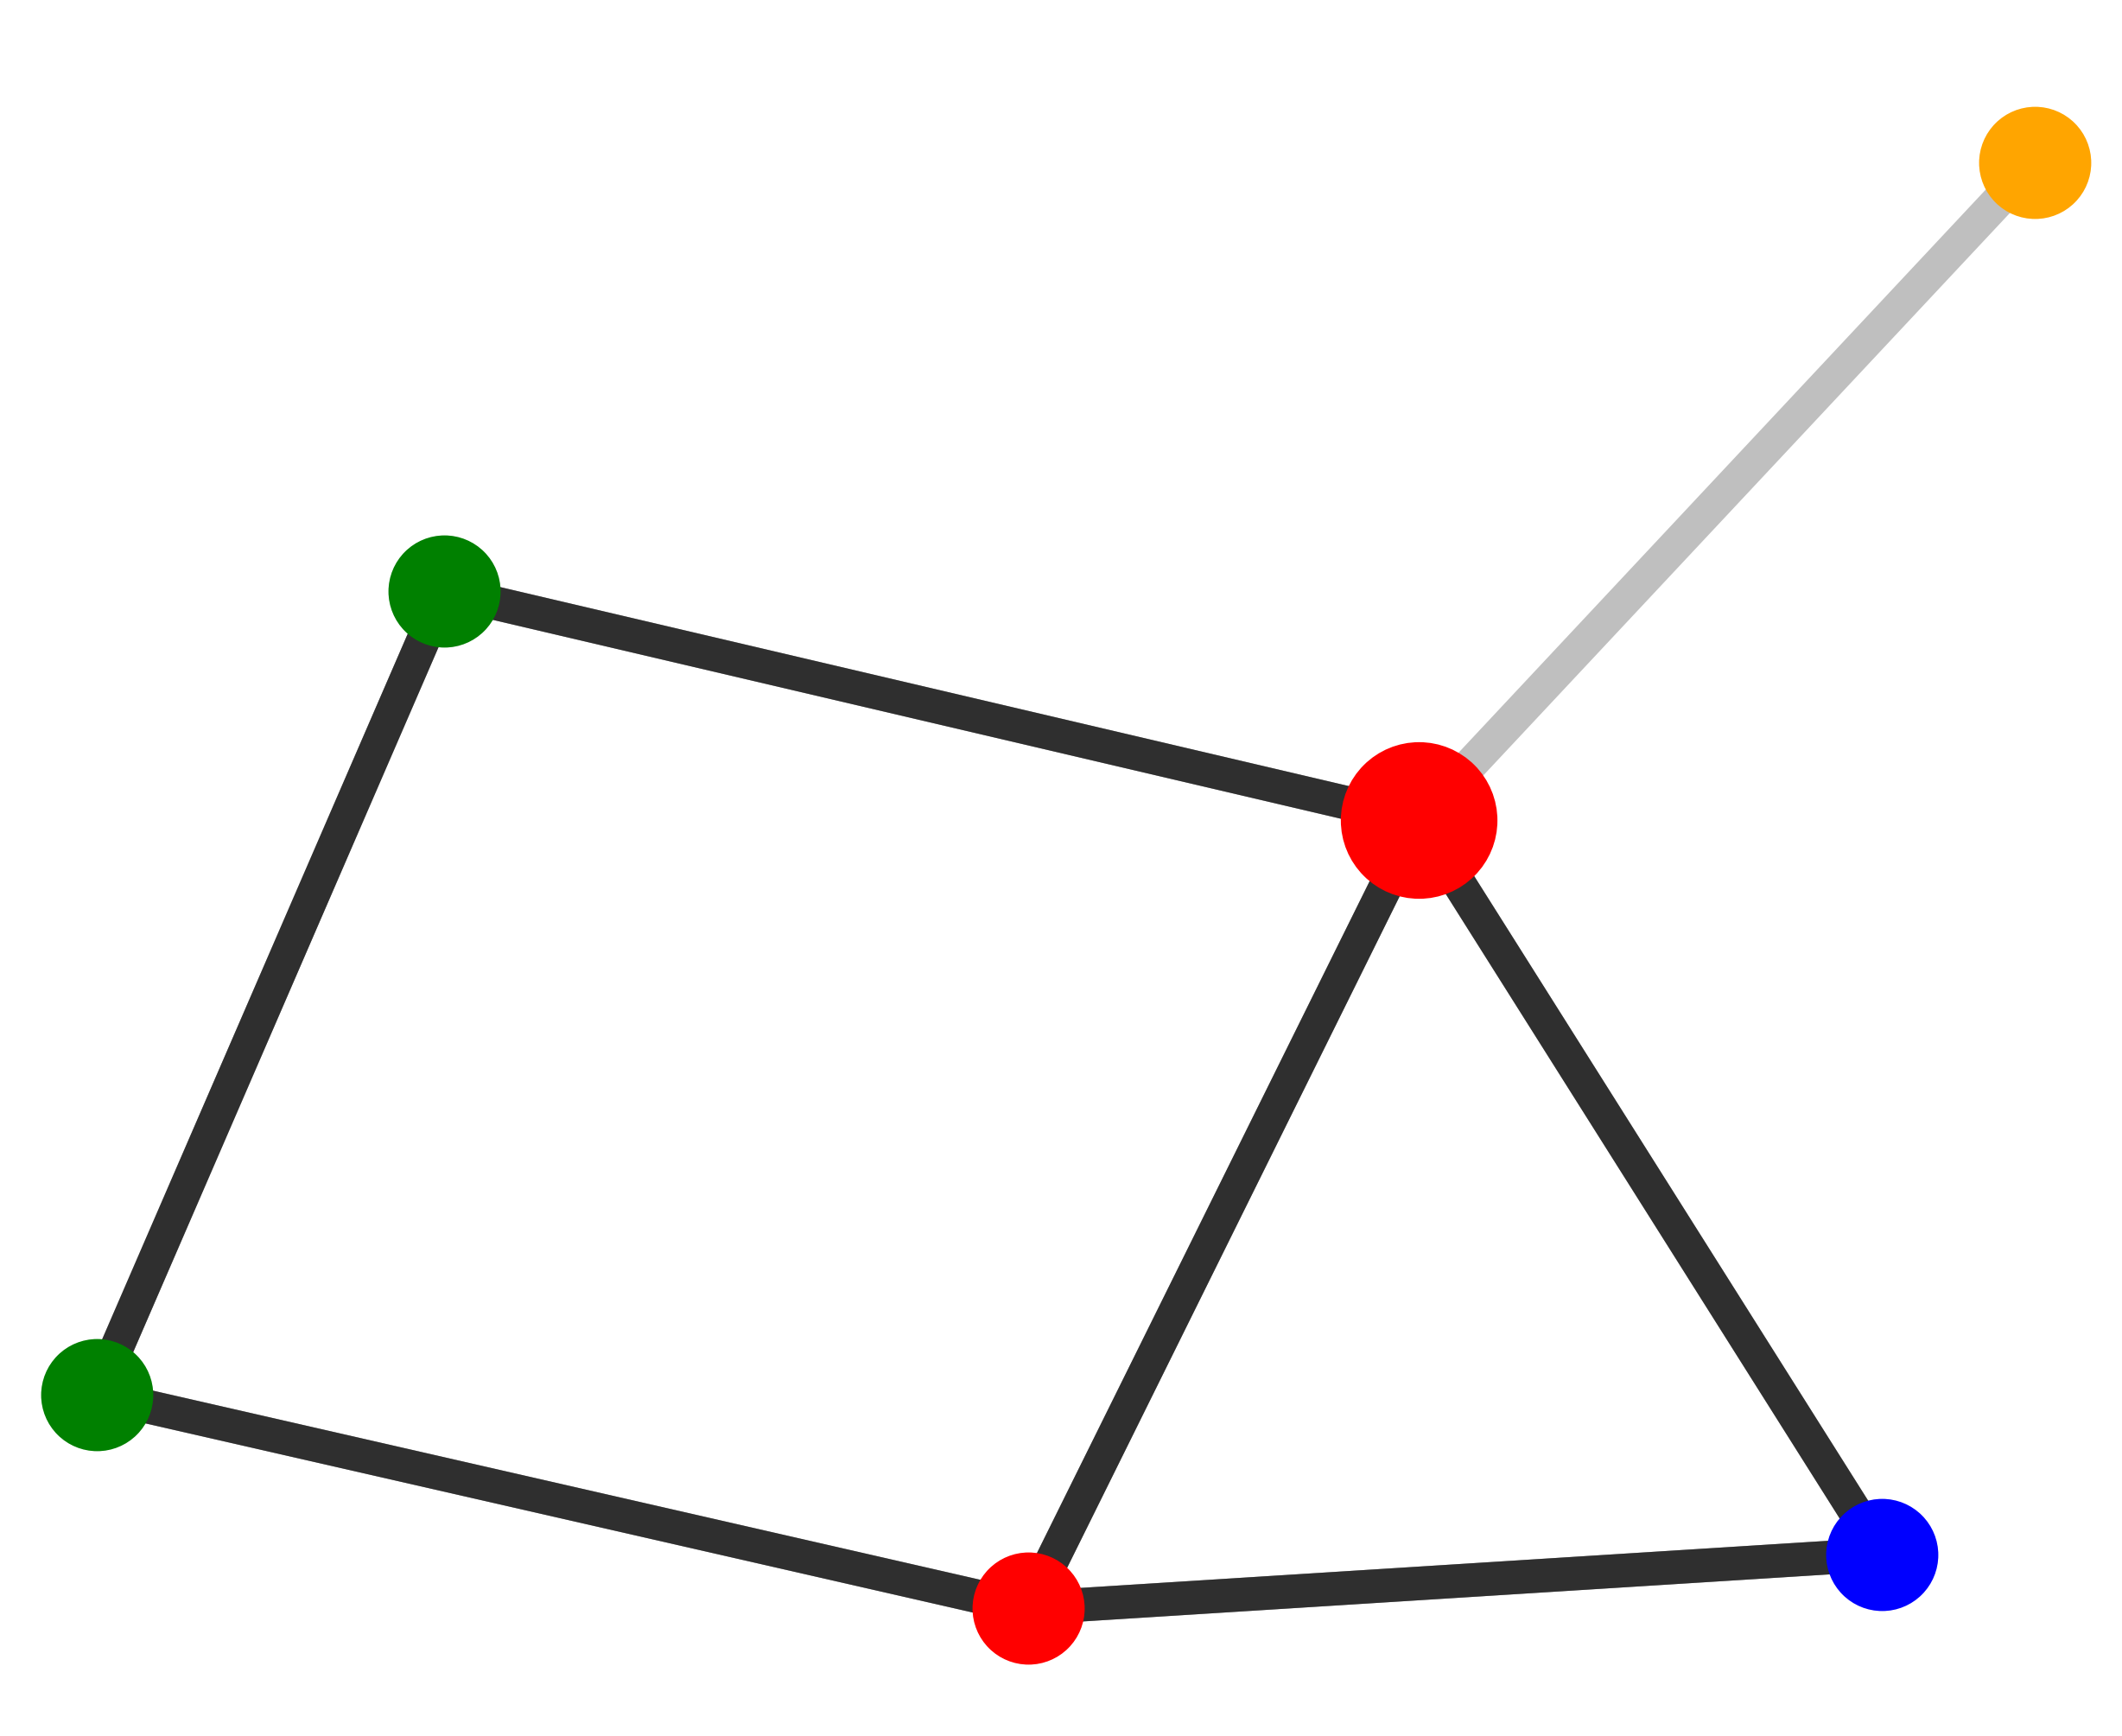
\includegraphics[width=.1\linewidth]{../openreview/imgs/their_image-1.png}
& 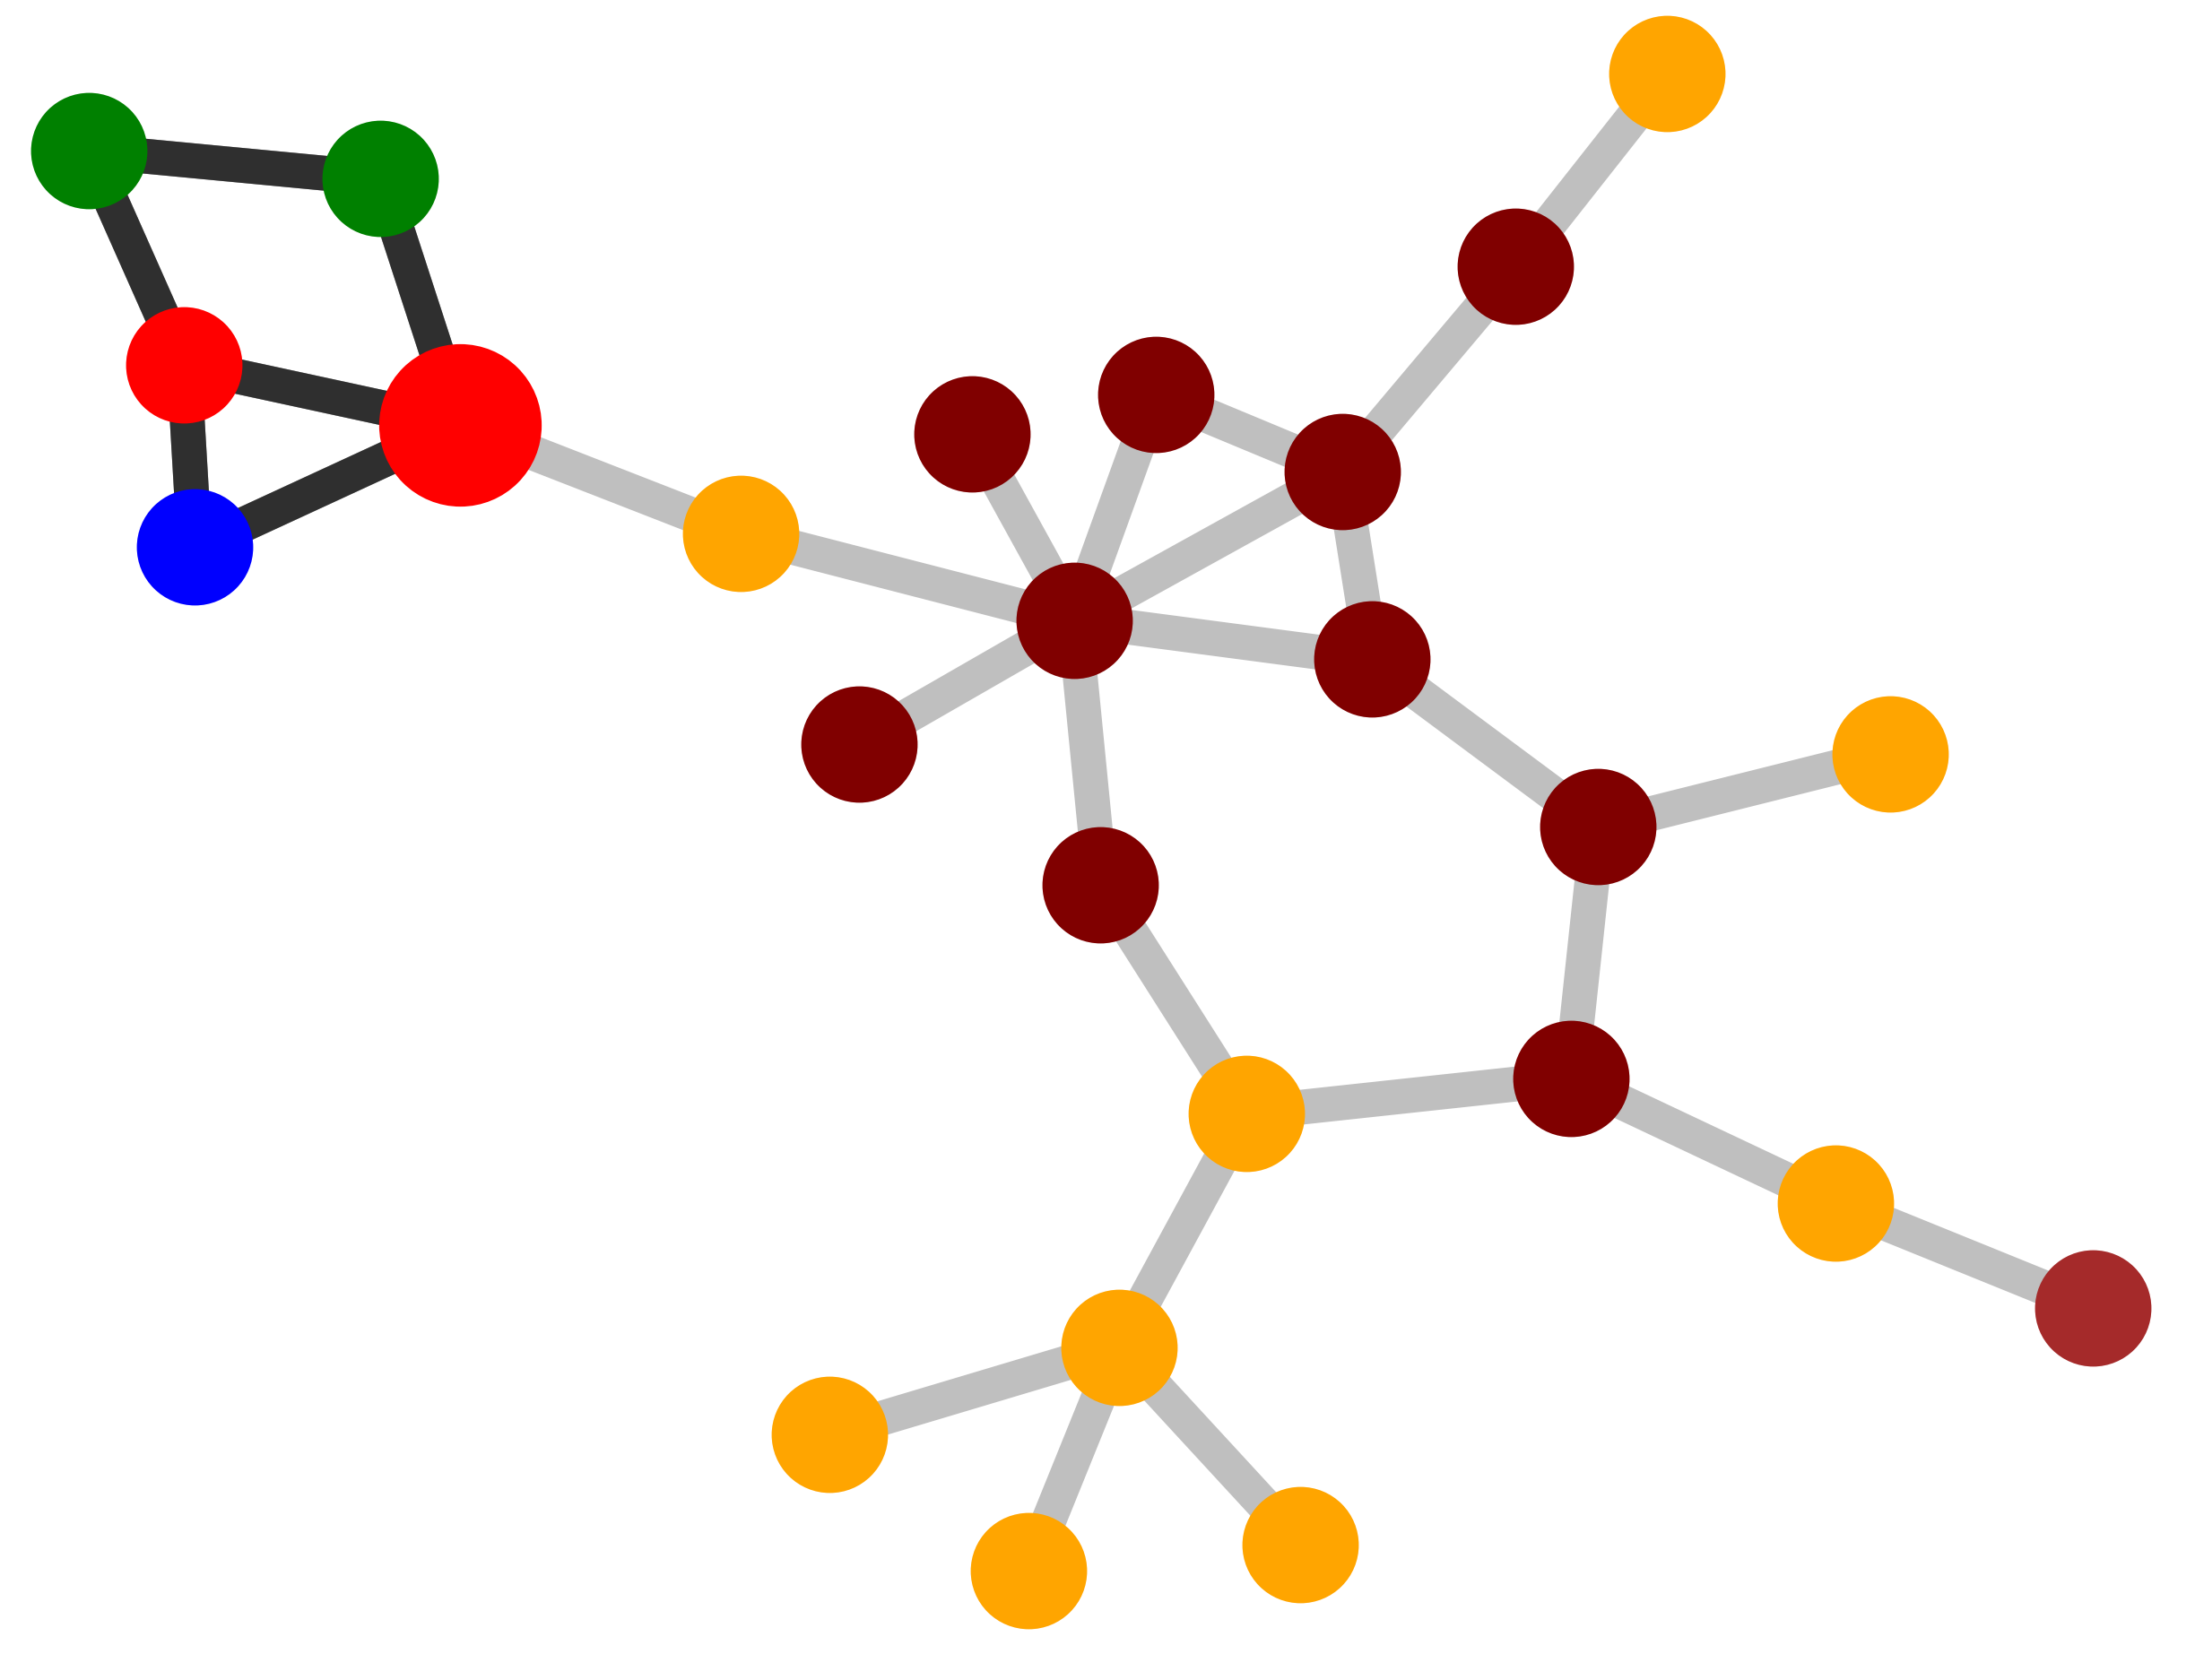
\includegraphics[width=.1\linewidth]{../openreview/imgs/their_image-2.png} & 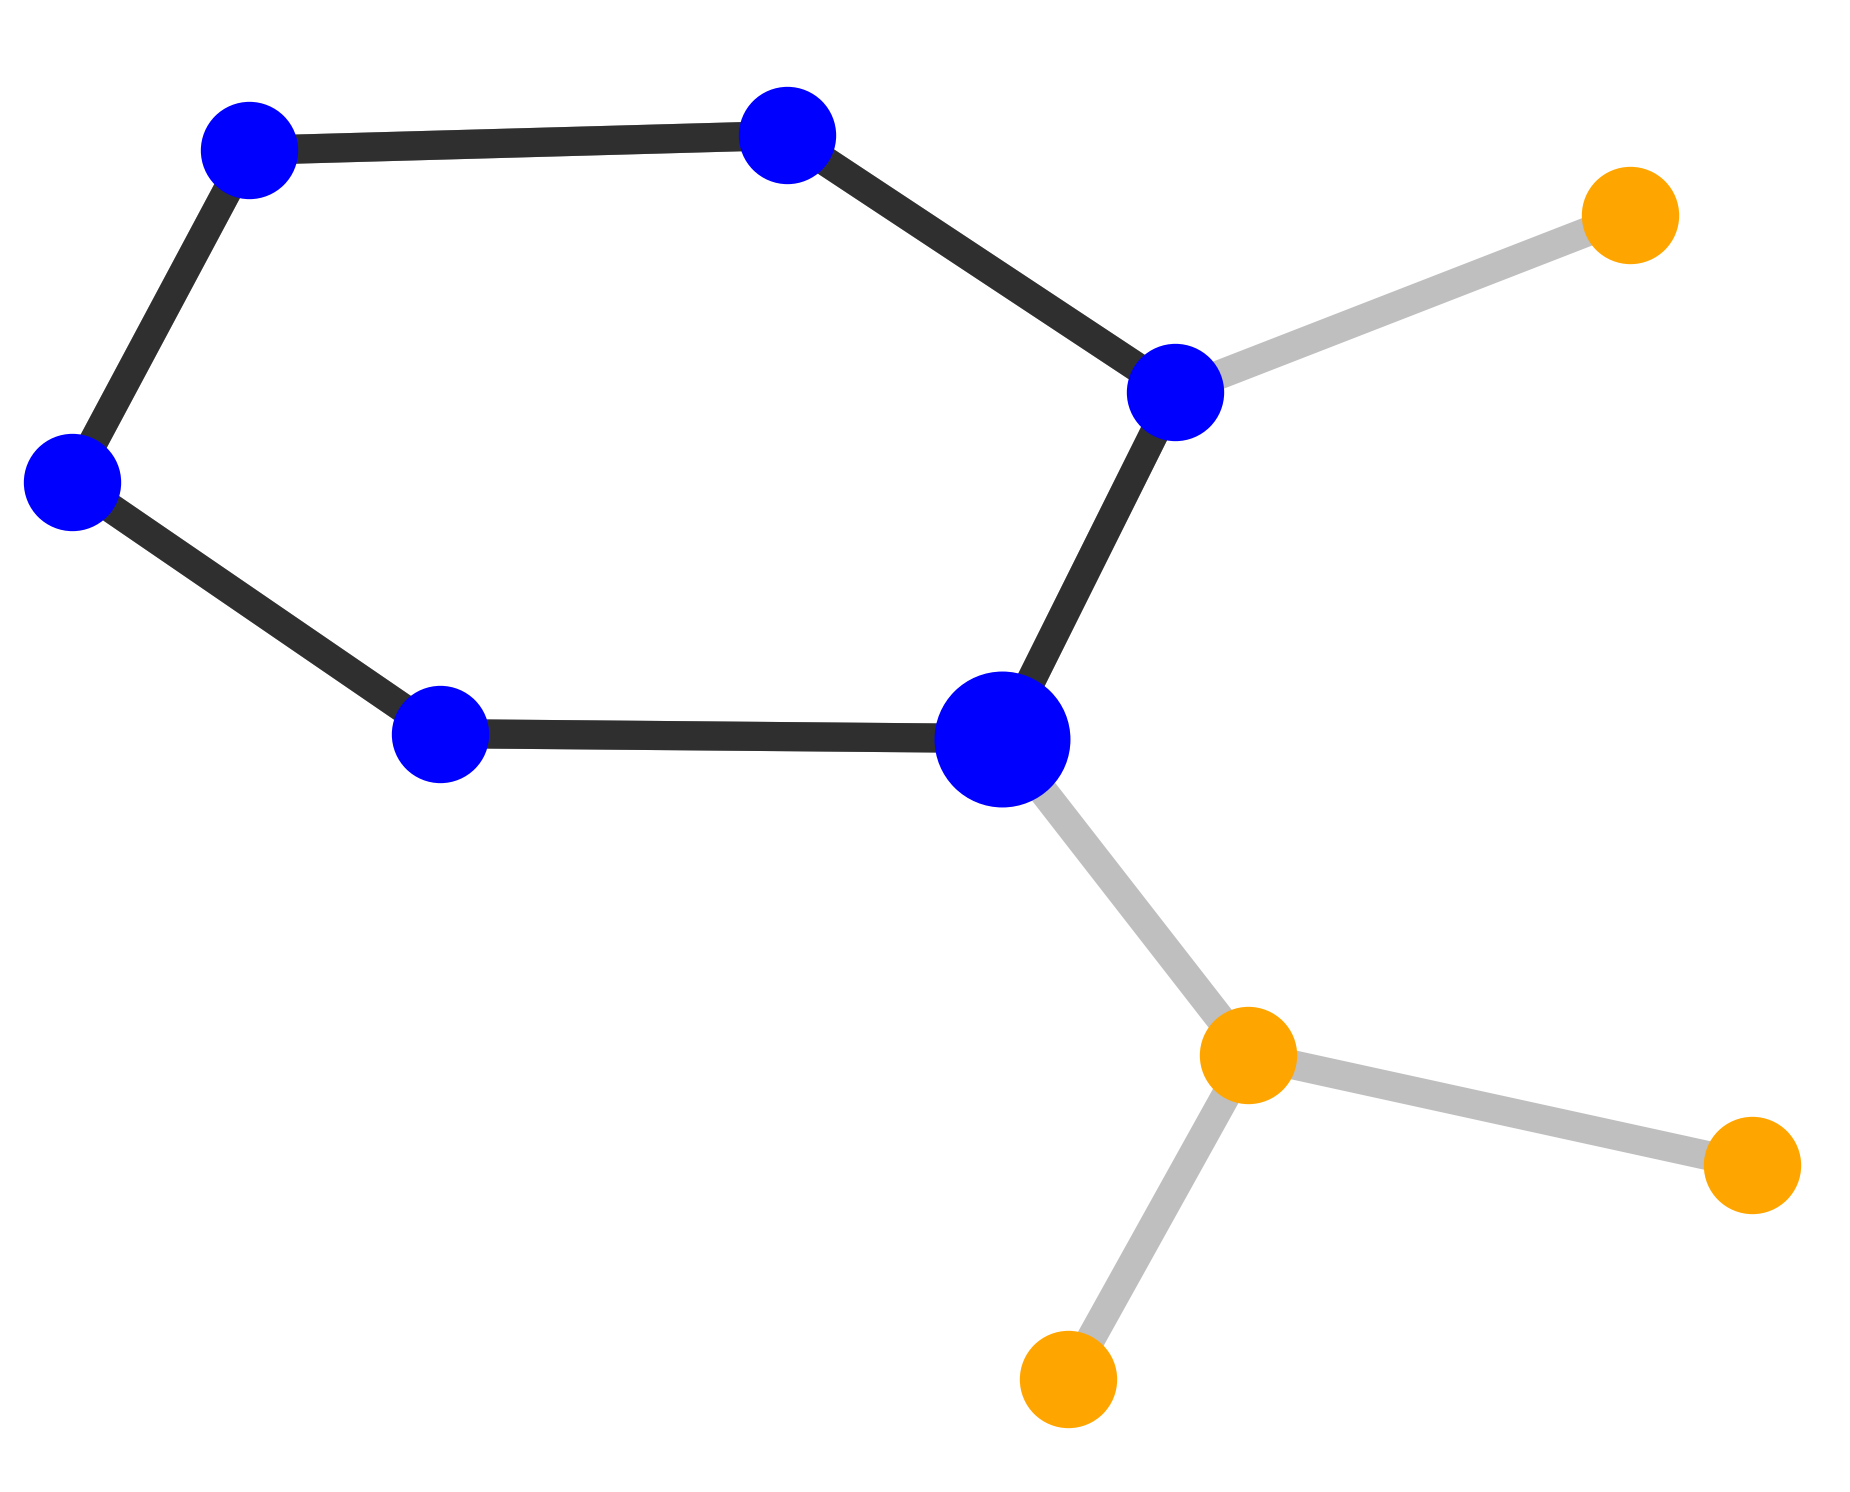
\includegraphics[width=.1\linewidth]{../openreview/imgs/their_image-3.png} & \multicolumn{1}{l}{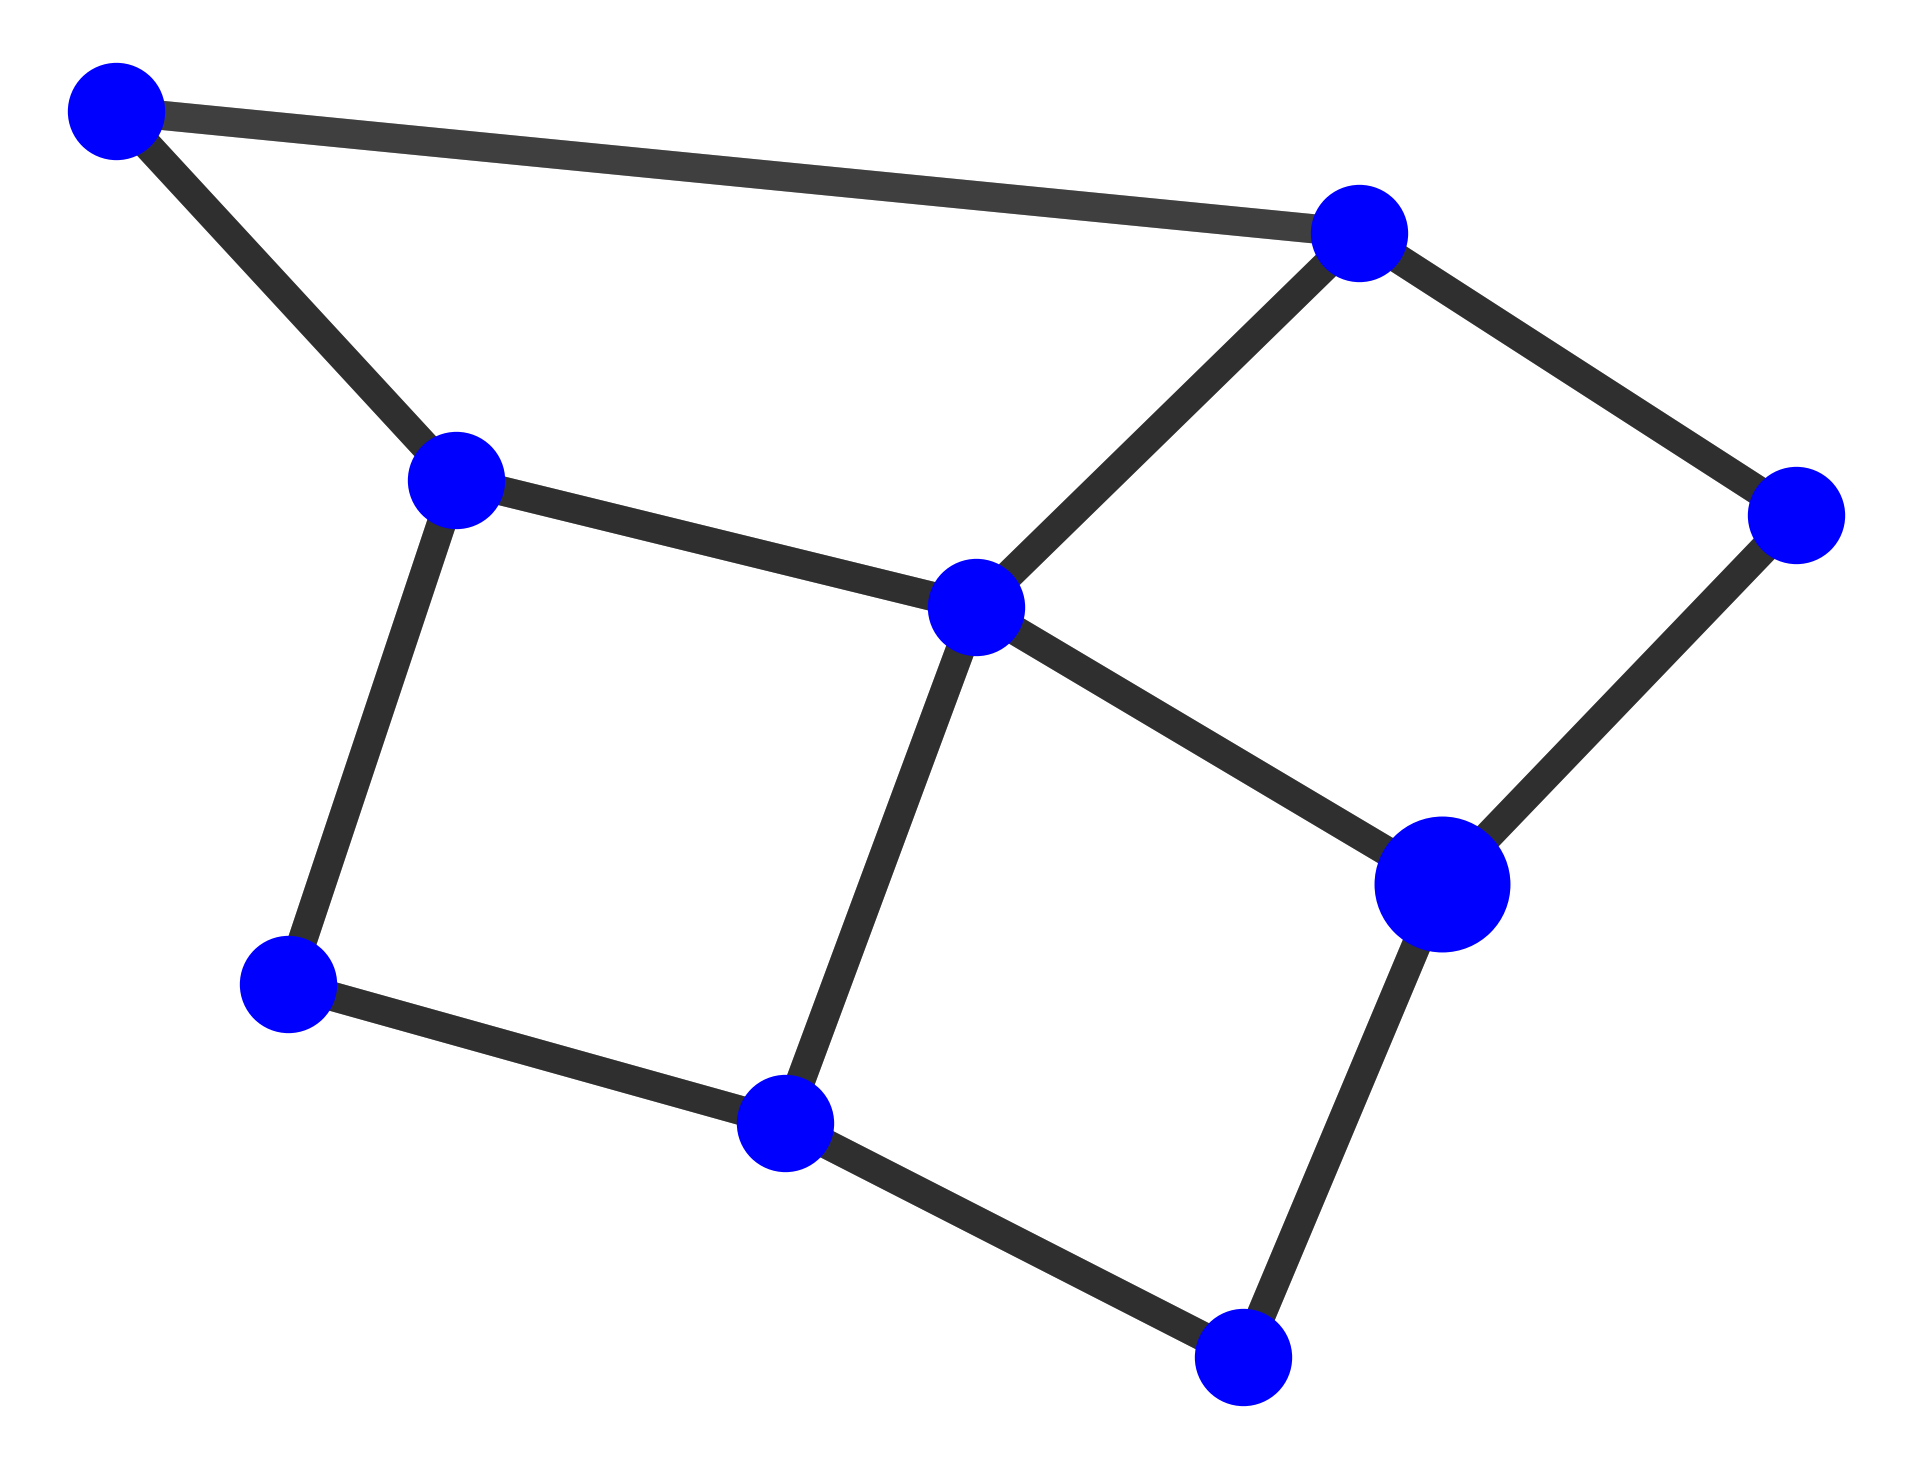
\includegraphics[width=.1\linewidth]{../openreview/imgs/their_image-4.png}} \\
No batch-norm &  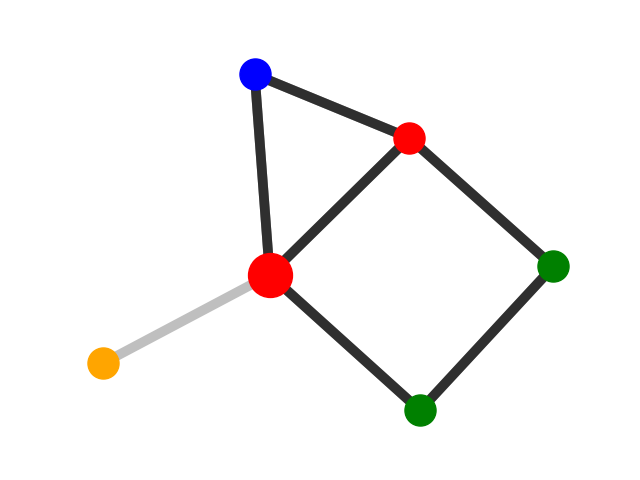
\includegraphics[width=.1\linewidth]{../openreview/imgs/simplification/syn1_pg.png}
& 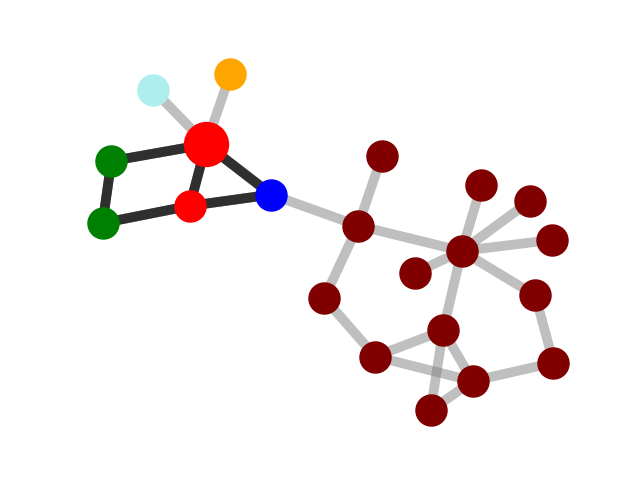
\includegraphics[width=.1\linewidth]{../openreview/imgs/simplification/syn2_pg.png} & 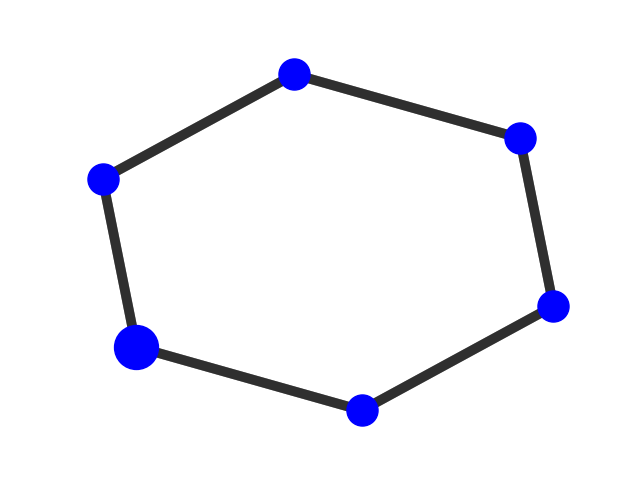
\includegraphics[width=.1\linewidth]{../openreview/imgs/simplification/syn3_pg.png} & \multicolumn{1}{l}{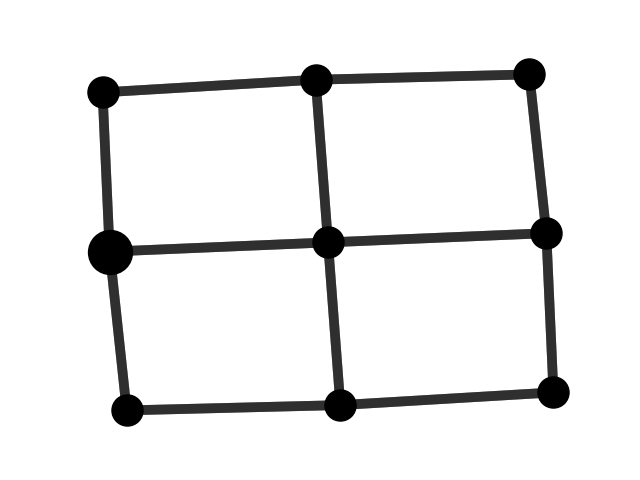
\includegraphics[width=.1\linewidth]{../openreview/imgs/simplification/syn4_pg.png}} \\
With batch-norm & 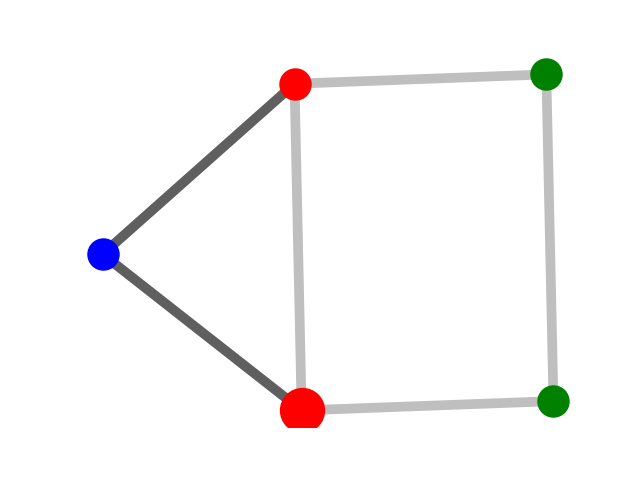
\includegraphics[width=.1\linewidth]{../openreview/imgs/replication/syn1.png}
& 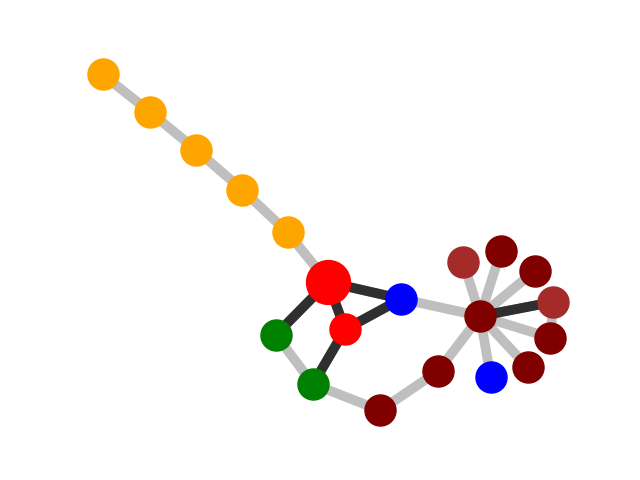
\includegraphics[width=.1\linewidth]{../openreview/imgs/replication/syn2.png} & 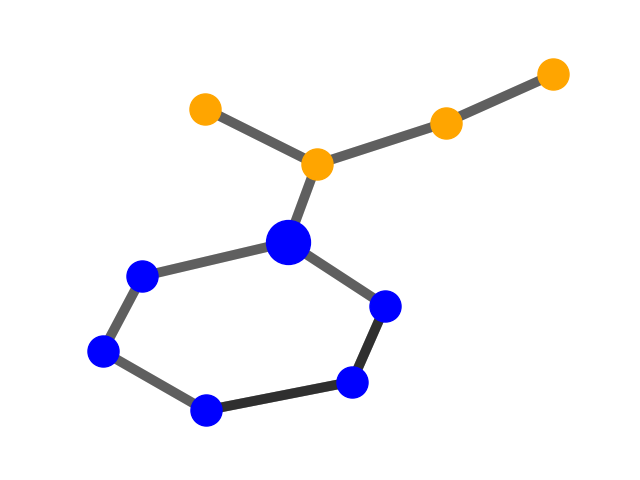
\includegraphics[width=.1\linewidth]{../openreview/imgs/replication/syn3.png} & \multicolumn{1}{l}{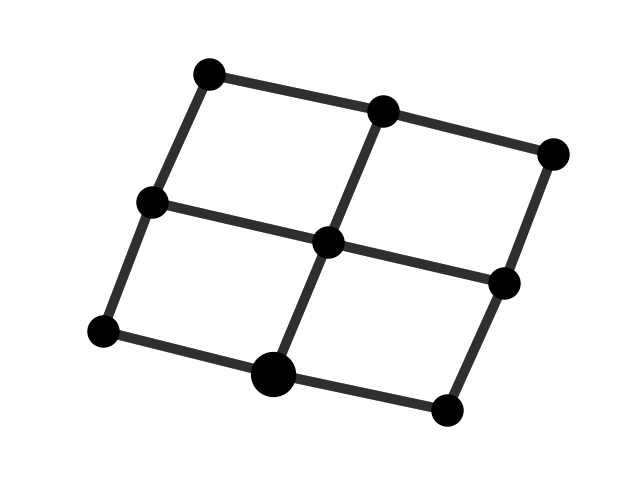
\includegraphics[width=.1\linewidth]{../openreview/imgs/replication/syn4.png}}  \\ \hline
\multicolumn{5}{l}{\textbf{Explanation AUC}} \\ \hline
Original & 0.963 ± 0.011 & 0.945 ± 0.019 & 0.987 ± 0.007 & \multicolumn{1}{l}{0.907 ± 0.014}  \\ 
No batch-norm & 0.999 ± 0.000 & 0.825 ± 0.040 & 0.760 ± 0.014 & \multicolumn{1}{l}{0.679 ± 0.008} \\
With batch-norm & 0.977 ± 0.006 & 0.970 ± 0.006 & 0.534 ± 0.186 & \multicolumn{1}{l}{0.649 ± 0.045}  \\ \hline
\multicolumn{5}{l}{\textbf{Inference Time (ms)}} \\ \hline
No batch-norm & 3.58 & 5.23 & 0.45 & \multicolumn{1}{l}{0.54} \\
With batch-norm & 3.56 & 5.29 & 0.40 & \multicolumn{1}{l}{0.47} \\ \bottomrule
\end{tabular}
\caption{Replicated experimental results from the quantitative, qualitative and efficiency study. For the qualitative visualization the samples are handpicked similar to the original paper. Node colors represent the node labels (if all colours are the same the nodes are unlabeled). Darkness of the edges signals importance for the final classification decision. In case of the node-classification datasets, the bigger node is the one for which the classification is being explained. For the quantitative explanation the average AUC score and standard deviation is given. The "original" row reports the PGExplainer AUC score from the original paper. The inference time reported represents the time needed to explain a single sample in milliseconds.}
\label{tab:reproduction_results}
\end{table}


\paragraph{Quantitative}
Quantitatively there is a significant difference between the explanations of the PGExplainer for models trained with or without batch normalization. However, the main conclusion based on these results remain the same. The replication experiments show that using the configuration provided in the codebase it is not possible to directly replicate the results presented in the paper. 


\paragraph{Qualitative}
No consistent significant difference in the visualized explanations can be observed between the two explained models. 

\paragraph{Efficiency}
The time required to explain the classification decision of a single node in the graph is consistent between the models trained with and without batch normalization. 

\section{Extended replication}\label{sec:extended_replication} 
In this extend replication we perform a simple experiment considering the issues raised in Sec.\,\ref{sec:3}. Specifically, we redo the quantitative evaluation of the synthetic node-classification using all test nodes instead of only those located in a motif. The model used for the explanation and the definition of the ground truth remains the same. 

\subsection{Results}
Quantitatively the PGExplainer scores significantly worse in the extended replication than during the original replication (see Tab.\,\ref{tab:extended_replication_results}). This is a direct result of performing the evaluation over the entire test set instead of only the nodes within a motif. The ground-truth for nodes outside the motif and the method used by both the GNNExplainer by PGExplainer are simply incompatible. 

Nevertheless, the improvement claimed by the authors of the PGExplainer over the GNNExplainer is still visible. Considering all datasets, the PGExplainer consistently outperforms the GNNExplainer by a significant margin. 

% \subsection{Experimental setup}
% For the extended reproduction the experimental setup is largely similar to the experimental setup of the replication, with the exemption of some notable improvements described below. Importantly, the dataset used are the same. 

% \subsubsection{Models}
% As described earlier, the model used for the replication is a direct copy of the model used in the GNNExplainer paper with the addition of the batch normalization that is kept in training mode during both training and evaluation. For the extended reproduction we revert this change and use an exact copy of the model used in the GNNExplainer instead. 

% A MODEL DEFINITION WILL FOLLOW HERE

% \subsubsection{Evaluation metrics}
% To extend the replication results, we focus on solving the issues discussed earlier. Hence, we will not be performing any additional experiments.

% \paragraph{Quantitative evaluation}
% To improve the quality of the quantitative evaluation, we lift a number of the restrictions imposed by the assumptions made in the original quantitative evaluation. First, and most importantly, the quantitative evaluation is not performed over the entire test set including those nodes and graphs that were excluded earlier because of not aligning with the idealistic ground-truths. 

% As we are still using the same data-sets, and therefore the same ground-truth definition, using the entire test set does raise some issues. For example, in the case of node-classifications all nodes outside of a motif have empty ground-truth explanations---ie. all surrounding edges have to be excluded from the explanation to achieve the maximum score. The same holds for the MUTAG dataset.

% Solving these issues would require a new definition of the ground-truth for graph datasets. For example, in the case of the tree-cycle dataset, one could define the ground-truth of a node outside a motif to be the entire 7-hop subgraph as this would be the minimal number of steps to take before one can conclude that no cycles have been formed. We however believe this to be outside the scope of this reproduction. 

% \paragraph{Qualitative evaluation}
% The main issue with the qualitative evaluation is the use of the hyper-parameter $k$. Ideally, an explanation method would determine this threshold based on a set of training samples, without the need of predefining it based on ground truth data. While it would be nice to do this for our extende reproduction, we believe that it would add a considerable additional functionality to the explainer the authors did not intend to have. For this reason, we will stick with the predefined values for $k$. \textit{IF WE HAVE TIME WE CAN TRY TO FIND THIS THRESHOLD AUTOMATICALLY. }

% A second issue is the arbitrary selection of the presented example. The original codebase accompanying the paper only produces a single visualized explanation for each dataset. Unfortunately this example is from the training set. Our updated implementation produces a visualized explanation for every single sample in the test set instead. In addition to this, when comparing the explanation for each model we do not only compare the best example from each explainer, but also their worst. 

% \paragraph{Efficiency}
% We extend the efficiency evaluation by also including the training time for the PGExplainer into the evaluation. The total time required to train is divided over all evaluated samples. 

% \subsection{Results}
% \paragraph{Model training}
% We find that there is not much of a difference between the models trained for the replication and those for the extended reproduction. Similar as before, the BA-community dataset overfits. 
% \begin{table}[]
% \centering
% \begin{tabular}{cccccccc}
% \toprule
% &\multicolumn{4}{c}{\textbf{Node Classification}} & \multicolumn{2}{c}{\textbf{Graph Classification}} \\
% Accuracy & \multicolumn{1}{c}{BA-Shapes} & \multicolumn{1}{c}{BA-Community} & \multicolumn{1}{c}{Tree-Cycles} & \multicolumn{1}{c|}{Tree-Grid} & \multicolumn{1}{c}{BA-2motifs} & \multicolumn{1}{c}{MUTAG} \\ 
% \midrule
% Training & 0.97 & 0.90 & 0.94 & \multicolumn{1}{c|}{0.96} & x.xx & 0.82 \\
% Validation & 1.00 & 0.75 & 0.98 & \multicolumn{1}{c|}{0.99} & x.xx & 0.82 \\
% Testing & 1.00 & 0.72 & 0.94 & \multicolumn{1}{c|}{0.99} & x.xx & 0.81 \\
% \bottomrule
% \end{tabular}
% \caption{Accuracies for the explained models used in the extended reproduction}
% \label{tab:accuracies_gnn}
% \end{table}

% \paragraph{Qualitative}
% In contrast to the replication, the qualitative part of the extended reproduction shows both a successful and a unsuccessful explanation for both the PGExplainer and the GNNExplainer. Explanation were deemed successful when they highlighted the datasets respective motif. This is similar to what is done in the original paper. Based on this notion of succesfulness, the good examples of explanations are in both the PGExplainer and GNNExplainer samples originating from nodes within the motif itself. The bad examples are nodes that are outside the motif. 

% \paragraph{Quantitative}
% Quantitatively the PGExplainer scores significantly worse in the extended evaluation then the replication. This is a direct result of performing the evaluation over the entire test set instead of only the nodes within a motif. The ground-truth for nodes outside the motif and the method used by both the GNNExplainer by PGExplainer are simply incompatible. 

% Nevertheless, the improvement claimed by the authors of the PGExplainer over the GNNExplainer is still visible. Considering all datasets, the PGExplainer consistently outperforms the GNNExplainer by a significant margin. 

% \paragraph{Efficiency}
% In terms of efficiency, the extended evaluation presents results consistent with the claims of the authors. The PGExplainer provies a considerable improvement in terms of inference time. This is despite our updated evaluation also taking the training time of the PGExplainer into account. 

\begin{table}[]
\centering
\begin{tabular}{lllll}
\toprule
\multicolumn{5}{c}{\textbf{Node Classification}} \\
\multicolumn{1}{c}{} & \multicolumn{1}{c}{BA-Shapes} & \multicolumn{1}{c}{BA-Community} & \multicolumn{1}{c}{Tree-Cycles} & \multicolumn{1}{c}{Tree-Grid} \\ \hline
\multicolumn{5}{l}{\textbf{Explanation AUC}} \\ \hline
PGExplainer & 0.974 ± 0.005 & 0.576 ± 0.024 & 0.748 ± 0.014 & \multicolumn{1}{l}{0.790 ± 0.009} \\
GNNExplainer & 0.508 ± 0.008 & 0.555 ± 0.002 & 0.482 ± 0.014 & \multicolumn{1}{l}{0.608 ± 0.009} \\ \bottomrule
\end{tabular}
\caption{Results of the extended replication study. For each explanation model both the AUC score over ten runs and the corresponding standard deviation is given. }
\label{tab:extended_replication_results}
\end{table}

% \subsection{Discussion}
% The results presented in the extended reproduction seem to be in line with the claims related to the GNNExplainer by the authors of the PGExplainer. Both in terms of accuracy and efficiency, the PGExplainer outperforms the GNNExplainer by a significant margin. However, the handling of ground-truth explanations remains inconsistent for the presented datasets. While the improvements in the evaluation pipeline, such as not using the training set for evaluation, might have improved the validity of the claims the usefulness of the used ground-truth explanations remain questionable. 

\section{Configuration}
Configuration files are used to provide a stable, flexible and reproducible way to run the experiments.
\subsection{Model configuration files}
The first type of configuration is the model configuration as seen in Fig.\,\ref{fig:model-config-example}, which contains (from top to bottom) the parameters required for training a GNN model. \texttt{dataset} assigns which dataset the model has to train on, \texttt{paper} defines which paper the model is build on (either PG, GNN or TAG), \texttt{lr} is the learning rate, \texttt{epochs} is the amount of epochs used for training and \texttt{clip\_max} is the parameter to which determines at what point the gradient is clipped. Additionally the file includes \texttt{early\_stopping} which defines the amount of epochs with no improvement that are required to enact early stopping of training, \texttt{seed} which defines the seed used for training and \texttt{eval\_enabled} which determines whether the model uses it's eval mode.
\begin{figure}[h!]
    \centering
    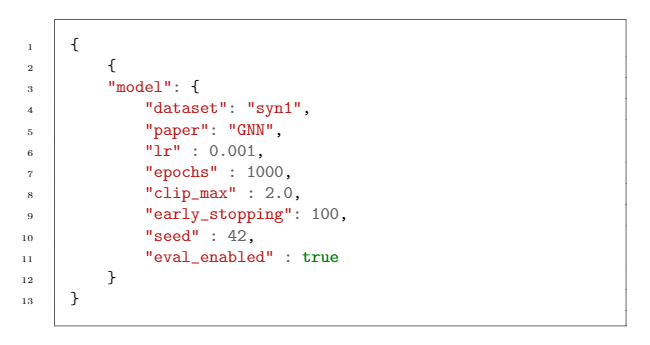
\includegraphics[width=0.5\textwidth]{../openreview/imgs/config-examples/model-config-example.png}
    \caption{Example of model config file in JSON format} 
\label{fig:model-config-example}
\end{figure}


\subsection{Explainer configuration files}
The second type of configuration is the explainer configuration an example of which is shown in Fig.\,\ref{fig:explainer-config-example}, these configuration files contain all parameters required to train an explainer and perform the the replication experiment using them. It includes the following parameters: \texttt{dataset} defines the dataset that the model that is to be explained is trained on. \texttt{model} is the type of model that has to be explainer, \texttt{explainer} is the implementation of the explainer (either PG or GNN). The configuration also contains the learning rate  and number of training epochs (\texttt{lr} and \texttt{epochs} respectively). As well as \texttt{sample\_bias} which determines the sample bias, the parameters \texttt{reg\_size} and \texttt{reg\_ent} that determine the size loss and entropy loss coefficients respectively, the temperatures, \texttt{seeds} the seeds used for training, \texttt{eval\_enabled} if the model uses evaluation mode and \texttt{thres\_snip} and \texttt{thres\_min} which define the thresholds for the interesting and sub-graph edges related to the drawing of the result explanations.  
\begin{figure}[h!]
    \centering
    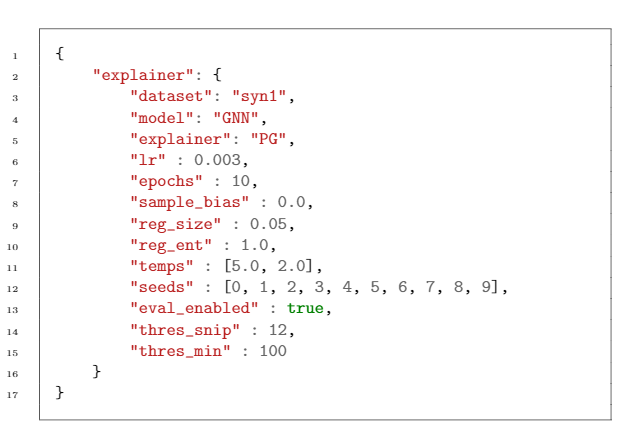
\includegraphics[width=0.5\textwidth]{../openreview/imgs/config-examples/explainer-config-example.png}
    \caption{Example of explainer configuration file in JSON format} 
\label{fig:explainer-config-example}
\end{figure}